\setmodule{9}

%BEGIN_FOLD % ====>>_____ Занятие 1 _____<<====
\begin{class}[number=1]
	\begin{listofex}
		%11.2,3,4 по 3 первых
		\item Найдите точку максимума функции \(y=x^3-48x+17\).
		\item Найдите наименьшее значение функции \(y=x^3-27x\) на отрезке \([0;4]\).
		\item Найдите наибольшее значение функции \(y=x^3-3x+4\) на отрезке \([-2;0]\).
		\item Найдите наименьшее значение функции \(y=\dfrac{ x^2+25 }{ x }\) на отрезке \([1;10]\).
		\item Найдите точку максимума функции \(y=-\dfrac{ x^2+289 }{ x }\).
		\item Найдите точку минимума функции \(y=-\dfrac{ x^2+1 }{ x }\).
		\item Найдите наименьшее значение функции \(y=(x-8)e^{x-7}\) на отрезке \([6;8]\).
		%11.5 1-4
		\item Найдите наименьшее значение функции \(y=3x-\ln (x+3)^3\) на отрезке \([-2,5;0]\).
		\item Найдите наибольшее значение функции \(y=\ln (x+5)^5-5x\) на отрезке \([-4,5;0]\).
		\item Найдите наименьшее значение функции \(y=4x-4\ln (x+7)+3\) на отрезке \([-6,5;0]\).
		\item Найдите наибольшее значение функции \(y=8\ln (x+5)-8x+54\) на отрезке \([-6,5;0]\).
		%11-trigon 1-3
		\item Найдите наименьшее значение функции \(y=5 \cos x - 6x + 4 \) на отрезке \( \left[ -\dfrac{ 3\pi }{ 2 }; 0 \right] \).
		\item Найдите наибольшее значение функции \(y=12\cos x + 6\sqrt{3}x - 2 \sqrt{3} \pi +6 \) на отрезке \( \left[ 0; \dfrac{ \pi }{ 2 } \right] \).
		\item Найдите наименьшее значение функции \(y=3+\dfrac{ 5\pi }{ 4 } -5x - 5\sqrt{2} \cos x \) на отрезке \( \left[ 0; \dfrac{ \pi }{ 2 } \right] \).
		
		\item Изюм получается в процессе сушки винограда. Сколько килограммов винограда потребуется для получения \(20\) килограммов изюма, если виноград содержит \(90\%\) воды, а изюм содержит \(5\%\) воды?
		
		%\item Изюм получается в процессе сушки винограда. Сколько килограммов винограда потребуется для получения \(16\) килограммов изюма, если виноград содержит \(90\%\) воды, а изюм содержит \(5\%\) воды?
		%BANK https://math-ege.sdamgia.ru/test?likes=99575 // https://math-ege.sdamgia.ru/test?likes=99576 // https://math-ege.sdamgia.ru/test?likes=99576 // https://math-ege.sdamgia.ru/test?likes=99578
		%по 2
		\item Имеется два сплава. Первый сплав содержит \(5\%\) меди, второй --- \(12\%\) меди. Масса второго сплава больше массы первого на \(9\) кг. Из этих двух сплавов получили третий сплав, содержащий \(10\%\) меди. Найдите массу третьего сплава. Ответ дайте в килограммах.
		%\item Имеется два сплава. Первый сплав содержит \(5\%\) меди, второй --- \(13\%\) меди. Масса второго сплава больше массы первого на \(9\) кг. Из этих двух сплавов получили третий сплав, содержащий \(10\%\) меди. Найдите массу третьего сплава. Ответ дайте в килограммах.
		
		\item Смешав \(11\)-процентный и \(72\)-процентный растворы кислоты и добавив \(10\) кг чистой воды, получили \(31\)-процентный раствор кислоты. Если бы вместо \(10\) кг воды добавили \(10\) кг \(50\)-процентного раствора той же кислоты, то получили бы \(51\)-процентный раствор кислоты. Сколько килограммов \(11\)-процентного раствора использовали для получения смеси?
		
		
		%\item Имеется два сплава. Первый содержит \(10\%\) никеля, второй --- \(35\%\) никеля. Из этих двух сплавов получили третий сплав массой \(150\) кг, содержащий \(30\%\) никеля. На сколько килограммов масса первого сплава была меньше массы второго?
		\item Имеется два сплава. Первый содержит \(15\%\) никеля, второй --- \(35\%\) никеля. Из этих двух сплавов получили третий сплав массой \(140\) кг, содержащий \(30\%\) никеля. На сколько килограммов масса первого сплава была меньше массы второго?
		
		
		\item Имеются два сосуда. Первый содержит \(30\) кг, а второй --- \(15\) кг раствора кислоты различной концентрации. Если эти растворы смешать, то получится раствор, содержащий \(34\%\) кислоты. Если же смешать равные массы этих растворов, то получится раствор, содержащий \(46\%\) кислоты. Сколько килограммов кислоты содержится в первом сосуде?
		
	\end{listofex}
\end{class}
%END_FOLD

%BEGIN_FOLD % ====>>_____ Занятие 2 _____<<====
\begin{class}[number=2]
	\begin{listofex}
		\item Занятие 2
	\end{listofex}
\end{class}
%END_FOLD

%BEGIN_FOLD % ====>>_ Домашняя работа 1 _<<====
\begin{homework}[number=1]
	\begin{listofex}
		%11.2,3 по 6-7 И 11.4 4-5
		\item Найдите наименьшее значение функции \(y=x^3-3x^2+2\) на отрезке \([1;4]\).
		\item Найдите наибольшее значение функции \(y=x^3-6x^2\) на отрезке \([-3;3]\).
		\item Найдите точку минимума функции \(y=\dfrac{ 25 }{ x }+x+25\).
		\item Найдите точку максимума функции \(y=-\dfrac{ x }{ x^2+9 }\).
		\item Найдите точку минимума функции \(y=(3-x)e^{3-x}\).
		\item Найдите наибольшее значение функции \(y=(x+16)e^{16-x}\) на отрезке \([15;17]\).
		%11-trigon 4-5
		\item Найдите наибольшее значение функции \( y=15x-3\sin x +5 \) на отрезке \( \left[ -\dfrac{ \pi }{ 2 }; 0 \right] \).
		\item Найдите наименьшее значение функции \( y=9 \cos x +14x + 7 \) на отрезке \( \left[ 0; \dfrac{ 3\pi }{ 2 } \right] \).
		\item Найдите радиус окружности, описанной около правильно треугольника со стороной \(3\).
		\item Найдите вписанный угол, опирающийся на дугу, которая составляет \(\dfrac{ 1 }{ 5 }\) от окружности. Ответ дайте в градусах.
		\item Периметр прямоугольника равен \(34\), а площадь равна \(60\). Найдите диагональ этого прямоугольника.
	\end{listofex}
\end{homework}
%END_FOLD

%BEGIN_FOLD % ====>>_____ Занятие 3 _____<<====
\begin{class}[number=3]
	\begin{listofex}
		\item 
		\begin{minipage}[t]{\bodywidth}
			Найдите площадь поверхности и объём куба, если его сторона равна \(3\sqrt{2}\) см.
		\end{minipage}
		\hspace{0.02\linewidth}
		\begin{minipage}[t]{\picwidth}
			\includegraphics[align=t, width=\linewidth]{\picpath/EGE2-cube}
		\end{minipage}
		\item 
		\begin{minipage}[t]{\bodywidth}
			Найдите площадь поверхности пространственного креста, изображенного на рисунке и составленного из кубов, сторона которого равна \(3\) см.
		\end{minipage}
		\hspace{0.02\linewidth}
		\begin{minipage}[t]{\picwidth}
			\includegraphics[align=t, width=\linewidth]{\picpath/EGE2-6cubes}
		\end{minipage}
		\item 
		\begin{minipage}[t]{\bodywidth}
			Найдите площадь поверхности многогранника, изображенного на рисунке (все двугранные углы прямые).
		\end{minipage}
		\hspace{0.02\linewidth}
		\begin{minipage}[t]{\picwidth}
			\includegraphics[align=t, width=\linewidth]{\picpath/EGE2-1}
		\end{minipage}
		
		\item 
		\begin{minipage}[t]{\bodywidth}
			Найдите объем и площадь поверхности многогранника, изображенного на рисунке (все двугранные углы прямые).
		\end{minipage}
		\hspace{0.02\linewidth}
		\begin{minipage}[t]{\picwidth}
			\includegraphics[align=t, width=\linewidth]{\picpath/EGE2-2}
		\end{minipage}
		\item В правильной треугольной пирамиде \(SABC\) медианы основания \(ABC \) пересекаются в точке \(O\). Площадь треугольника \(ABC\) равна \(2\); объем пирамиды равен \(5\). Найдите длину отрезка \(OS\).
		%\item В сосуд, имеющий форму правильной треугольной призмы, налили \(2300\) см\(^3\) воды и погрузили в воду деталь. При этом уровень воды поднялся с отметки \(25\) см до отметки \(27\) см. Найдите объем детали. Ответ выразите в см\(^3\).
		%\item Найдите объём и площадь поверхности прямой призмы, в основании которой лежит ромб с диагоналями, равными \(6\) и \(8\), а боковое ребро призмы равно 10.
		\item От треугольной призмы, объем которой равен \(6\), отсечена треугольная пирамида плоскостью, проходящей через сторону одного основания и противоположную вершину другого основания. Найдите объем оставшейся части.
		\item 
		\begin{minipage}[t]{\bodywidth}
			Объём куба равен \(12\). Найдите объём треугольной призмы, отсекаемой от куба плоскостью, проходящей через середины двух рёбер, выходящих из одной вершины, и параллельной третьему ребру, выходящему из этой же вершины.
		\end{minipage}
		\hspace{0.02\linewidth}
		\begin{minipage}[t]{\picwidth}
			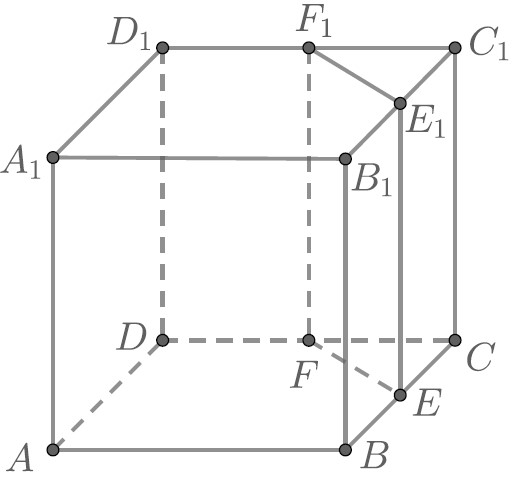
\includegraphics[align=t, width=\linewidth]{\picpath/prob_1_4}
		\end{minipage}
		\item 
		\begin{minipage}[t]{\bodywidth}
			Объем параллелепипеда \(ABCDA_1B_1C_1D_1\) равен \(4,5\). Найдите объем треугольной пирамиды \(AD_1CB_1\).
		\end{minipage}
		\hspace{0.02\linewidth}
		\begin{minipage}[t]{\picwidth}
			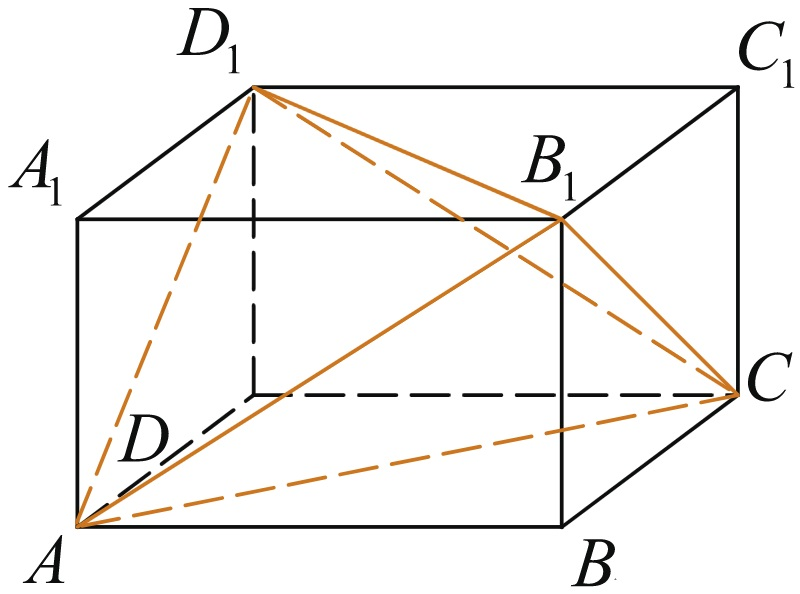
\includegraphics[align=t, width=\linewidth]{\picpath/G112M8L3-1}
		\end{minipage}
		
		\item 
		\begin{minipage}[t]{\bodywidth}
			Объем параллелепипеда \(ABCDA_1B_1C_1D_1\) равен \(9\). Найдите объем треугольной пирамиды \(ABCA_1\).
		\end{minipage}
		\hspace{0.02\linewidth}
		\begin{minipage}[t]{\picwidth}
			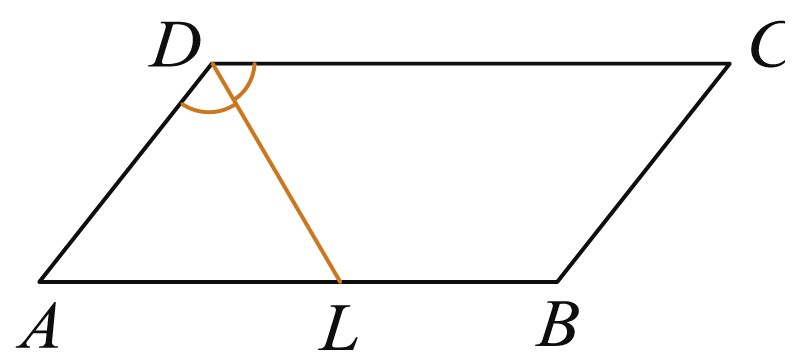
\includegraphics[align=t, width=\linewidth]{\picpath/prob_3_1}
		\end{minipage}
		
		
		%\item Шар вписан в цилиндр. Площадь полной поверхности цилиндра равна \(18\). Найдите площадь поверхности шара.
		\item Прямоугольный параллелепипед описан около цилиндра, радиус основания и высота которого равны \(1\). Найдите объем параллелепипеда.
		\item Цилиндр и конус имеют общие основание и высоту. Найдите объем конуса, если объем цилиндра равен \(150\).
		\item Объем конуса равен \(16\). Через середину высоты параллельно основанию конуса проведено сечение, которое является основанием меньшего конуса с той же вершиной. Найдите объем меньшего конуса.
		\item Во сколько раз увеличится объем конуса, если радиус его основания увеличится в \(1,5\) раза, а высота останется прежней?
		\item Во сколько раз уменьшится объем конуса, если его высота уменьшится в \(3\) раза, а радиус основания останется прежним?
		\item Во сколько раз увеличится площадь боковой поверхности конуса, если его образующая увеличится в \(3\) раза, а радиус основания останется прежним?
		\item Площадь боковой поверхности конуса в два раза больше площади основания. Найдите угол между образующей конуса и плоскостью основания. Ответ дайте в градусах.
		\item Площадь основания конуса равна \(16\pi \), высота --- \(6\). Найдите площадь осевого сечения конуса.
		\item Диаметр основания конуса равен \(6\), а угол при вершине осевого сечения равен \(90\degree \). Вычислите объем конуса, деленный на \(\pi\).
		
		
		
	\end{listofex}
\end{class}
%END_FOLD

%BEGIN_FOLD % ====>>_____ Занятие 4 _____<<====
\begin{class}[number=4]
	\begin{listofex}
		\item Занятие 4
	\end{listofex}
\end{class}
%END_FOLD

%BEGIN_FOLD % ====>>_ Домашняя работа 2 _<<====
\begin{homework}[number=2]
	\begin{listofex}
		\item Высота конуса равна \(4\), а диаметр основания --- \(6\). Найдите образующую конуса.
		\item Площадь основания конуса равна \(16\pi \), высота --- \(6\). Найдите площадь осевого сечения конуса.
		\item Длина окружности основания цилиндра равна \(3\). Площадь боковой поверхности равна \(6\). Найдите высоту цилиндра.
		\item Площадь боковой поверхности цилиндра равна \(2\pi \) , а высота  --- \(1\). Найдите диаметр основания.
		\item Площадь поверхности шара равна \(24\). Найдите площадь большого круга шара.
		\item Во сколько раз уменьшится объем конуса, если его высота уменьшится в \(10\) раз, а радиус основания останется прежним?
		\item Во сколько раз увеличится площадь боковой поверхности конуса, если его образующая увеличится в \(6\) раз, а радиус основания останется прежним?
		\item Площадь поверхности правильной треугольной призмы равна \(6\). Какой станет площадь поверхности призмы, если все её рёбра увеличатся в три раза, а форма останется прежней?
		
		\item Изюм получается в процессе сушки винограда. Сколько килограммов винограда потребуется для получения \(82\) килограммов изюма, если виноград содержит \(90\%\) воды, а изюм содержит \(5\%\) воды?
		\item Смешав \(55\)-процентный и \(97\)-процентный растворы кислоты и добавив \(10\) кг чистой воды, получили \(65\)-процентный раствор кислоты. Если бы вместо \(10\) кг воды добавили \(10\) кг \(50\)-процентного раствора той же кислоты, то получили бы \(75\)-процентный раствор кислоты. Сколько килограммов \(55\)-процентного раствора использовали для получения смеси?
		\item Имеются два сосуда. Первый содержит \(100\) кг, а второй --- \(20\) кг раствора кислоты различной концентрации. Если эти растворы смешать, то получится раствор, содержащий \(67\%\) кислоты. Если же смешать равные массы этих растворов, то получится раствор, содержащий \(77\%\) кислоты. Сколько килограммов кислоты содержится в первом сосуде?
	\end{listofex}
\end{homework}
%END_FOLD

%BEGIN_FOLD % ====>>_____ Занятие 5 _____<<====
\begin{class}[number=5]
	\begin{listofex}
		\item Занятие 5
	\end{listofex}
\end{class}
%END_FOLD

%BEGIN_FOLD % ====>>_____ Занятие 6 _____<<====
\begin{class}[number=6]
	\begin{listofex}
		\item Занятие 6
	\end{listofex}
\end{class}
%END_FOLD

%BEGIN_FOLD % ====>>_ Домашняя работа 3 _<<====
\begin{homework}[number=3]
	\begin{listofex}
		\item Домашняя работа 3
	\end{listofex}
\end{homework}
%END_FOLD

%BEGIN_FOLD % ====>>_____ Занятие 7 _____<<====
\begin{class}[number=7]
	\title{Подготовка к проверочной}
	\begin{listofex}
		\item Занятие 7
	\end{listofex}
\end{class}
%END_FOLD

%BEGIN_FOLD % ====>>_ Проверочная работа _<<====
\begin{exam}
	\begin{listofex}
		\item Проверочная
	\end{listofex}
\end{exam}
%END_FOLD

%BEGIN_FOLD % ====>>_ Консультация Борисов _<<====
\begin{consultation}
	\begin{listofex}
		\item Найдите площадь треугольника, две стороны которого равны \(8\) и \(12\), а угол между ними равен \(30 \degree\).
		\item Большее основание равнобедренной трапеции равно \(34\). Боковая сторона равна \(14\). Синус острого угла равен \( \dfrac{ 2\sqrt{10}}{ 7 } \). Найдите меньшее основание.
		%\item Основания равнобедренной трапеции равны \(7\) и \(51\). Тангенс острого угла равен \( \dfrac{ 5 }{ 11 } \).  Найдите высоту трапеции.
		%\item Большее основание равнобедренной трапеции равно \(34\). Боковая сторона равна \(14\). Синус острого угла равен \( \dfrac{ 2\sqrt{10}}{ 7 } \). Найдите меньшее основание.
		\item Основания равнобедренной трапеции равны \(7\) и \(51\). Тангенс острого угла равен \( \dfrac{ 5 }{ 11 } \).  Найдите высоту трапеции.
		\item В параллелограмме \( ABCD: \quad AB  =  3, AD  =  21, \sin A = \dfrac{ 6 }{ 7 } \). Найдите большую высоту параллелограмма.
		\item Найдите площадь ромба, если его высота равна \(2\), а острый угол \(30\degree \).
		\item Периметр треугольника равен \(12\), а радиус вписанной окружности равен \(1\). Найдите площадь этого треугольника.
		\item Найдите радиус окружности, вписанной в правильный треугольник, высота которого равна \(6\).
		\item Сторона правильного треугольника равна \(\sqrt{3}\). Найдите радиус окружности, описанной около этого треугольника.
		\item Найдите сторону правильного шестиугольника, описанного около окружности, радиус которой равен \(\sqrt{3}\).
		\item Чему равна сторона правильного шестиугольника, вписанного в окружность, радиус которой равен \(6\)?
		\item Даны два шара. Радиус первого шара в \(2\) раза больше радиуса второго. Во сколько раз площадь поверхности первого шара больше площади поверхности второго?
		\item Шар вписан в цилиндр. Площадь полной поверхности цилиндра равна \(18\). Найдите площадь поверхности шара.
		\item Прямоугольный параллелепипед описан около цилиндра, радиус основания и высота которого равны \(1\). Найдите объем параллелепипеда.
		\item Объем первого цилиндра равен \(12\) м\(^3\). У второго цилиндра высота в три раза больше, а радиус основания --- в два раза меньше, чем у первого. Найдите объем второго цилиндра. Ответ дайте в кубических метрах.
		\item В цилиндрический сосуд налили \(2000\) см\(^3\) воды. Уровень воды при этом достигает высоты \(12\) см. В жидкость полностью погрузили деталь. При этом уровень жидкости в сосуде поднялся на \(9\) см. Чему равен объем детали? Ответ выразите в см\(^3\).
		\item Объем конуса равен \(16\). Через середину высоты параллельно основанию конуса проведено сечение, которое является основанием меньшего конуса с той же вершиной. Найдите объем меньшего конуса.
		\item В сосуд, имеющий форму правильной треугольной призмы, налили \(2300\) см\(^3\) воды и погрузили в воду деталь. При этом уровень воды поднялся с отметки \(25\) см до отметки \(27\) см. Найдите объем детали. Ответ выразите в см\(^3\).
	\end{listofex}
\end{consultation}

%BEGIN_FOLD % ====>>_ Консультация Борисов _<<====
\begin{consultation}
	\begin{listofex}
		%???chelnokovam5
		\item Вычислить: 
		\begin{tasks}(2)
			\task \( \dfrac{5\cos29\degree}{\sin61\degree} \)
			\task \( -4\sqrt{3}\cos(-750\degree) \)
			\task \( \dfrac{4\cos146\degree}{\cos34\degree} \)
			\task \( 7\tg13\degree\cdot\tg77\degree \)
			\task \( \dfrac{12}{\sin^227\degree+\cos^2207\degree} \)
			\task \( \dfrac{5\sin98\degree}{\sin49\degree\cdot\sin41\degree} \)
			\task \( -50\tg9\degree\cdot\tg81\degree+31 \)
		\end{tasks}
		\item Вычислить: %114m3
		\begin{tasks}(2)
			\task \( \dfrac{-13\sin126\degree}{\sin54\degree} \)
			\task \( \cos^2(-46\degree)+\sin^2(-46\degree) \)
			\task \( \sin^223\degree+9+\cos^223 \)
			\task \( \dfrac{2\sin^221\degree+2\cos^221\degree}{4} \)
		\end{tasks}
		%n5 cos1
		\item Найдите корни уравнения: \( \cos \dfrac{ \pi(x-7) }{ 3 } = 0,5 \).  В ответ запишите наибольший отрицательный корень.
		%n5 cos3
		\item Найдите корни уравнения: \( \cos \dfrac{ \pi(2x+9) }{ 3 } = \dfrac{ \sqrt{2} }{ 2 } \).  В ответ запишите наибольший отрицательный корень.
		%n5 sin1
		\item Найдите корни уравнения: \( \sin \dfrac{ \pi x }{ 3 } = 0,5 \).  В ответ запишите наименьший положительный корень.
		%n5 tg1
		\item Найдите корни уравнения: \( \tg \dfrac{ \pi x }{ 4 } = -1 \).  В ответ запишите наибольший отрицательный корень.
		%n5 tg2
		\item Найдите корни уравнения: \( \tg \dfrac{ \pi (x+2) }{ 3 } = -\sqrt{3} \).  В ответ запишите наибольший отрицательный корень.
		\item Найдите: %101L1
		\begin{tasks}
			\task \( 5\sin\alpha \), если \( \cos\alpha=\dfrac{2\sqrt{6}}{5} \) и \( \alpha\in\left( \dfrac{3\pi}{2}; 2\pi \right) \);
			\task \( 3\cos\alpha \), если \( \sin\alpha=-\dfrac{2\sqrt{2}}{3} \) и \( \alpha\in\left( \dfrac{3\pi}{2}; 2\pi \right) \);
			\task \( 24\cos\alpha \), если \( \sin\alpha=-0,2 \);
			\task \( \sin\left( \dfrac{7\pi}{2}-\alpha \right) \), если \( \sin\alpha=0,8 \) и \( \alpha\in\left( \dfrac{\pi}{2}; \pi \right) \).
		\end{tasks}
		\item При нормальном падении света с длиной волны \( \lambda=400 \) нм на дифракционную решeтку с периодом \(d\) нм наблюдают серию дифракционных максимумов. При этом угол \(\varphi\)  (отсчитываемый от перпендикуляра к решeтке), под которым наблюдается максимум, и номер максимума \(k\) связаны соотношением \(d \sin \varphi= k\lambda\). Под каким минимальным углом \(\varphi\) (в градусах) можно наблюдать второй максимум на решeтке с периодом, не превосходящим \(1600\) нм?
		%priklad trigon 2
		\item Два тела массой \(m=2\) кг каждое, движутся с одинаковой скоростью  \(v =10\) м/с под углом \(2\alpha\) друг к другу. Энергия (в джоулях), выделяющаяся при их абсолютно неупругом соударении определяется выражением \(Q= m v^2 \sin^2 \alpha \). Под каким наименьшим углом \(2\alpha\) (в градусах) должны двигаться тела, чтобы в результате соударения выделилось не менее \(50\) джоулей?
	\end{listofex}
\end{consultation}
